\chapter{应用性能优化}
\label{cha:ApplicationOptimization}
\section{Couchbase缓存优化}
目前大多数的WEB应用产品在设计开发的过程中对数据的读取还依旧通过直接对数据库进行增、删、改、查来实现。然而随着用户数量的增加,用户的请求也不断的增多,这对于数据库的压力是非常大的。之前的数据操作流程参见图~\ref{fig:couchbase1}。
\begin{figure}[H] % use float package if you want it here
  \centering
  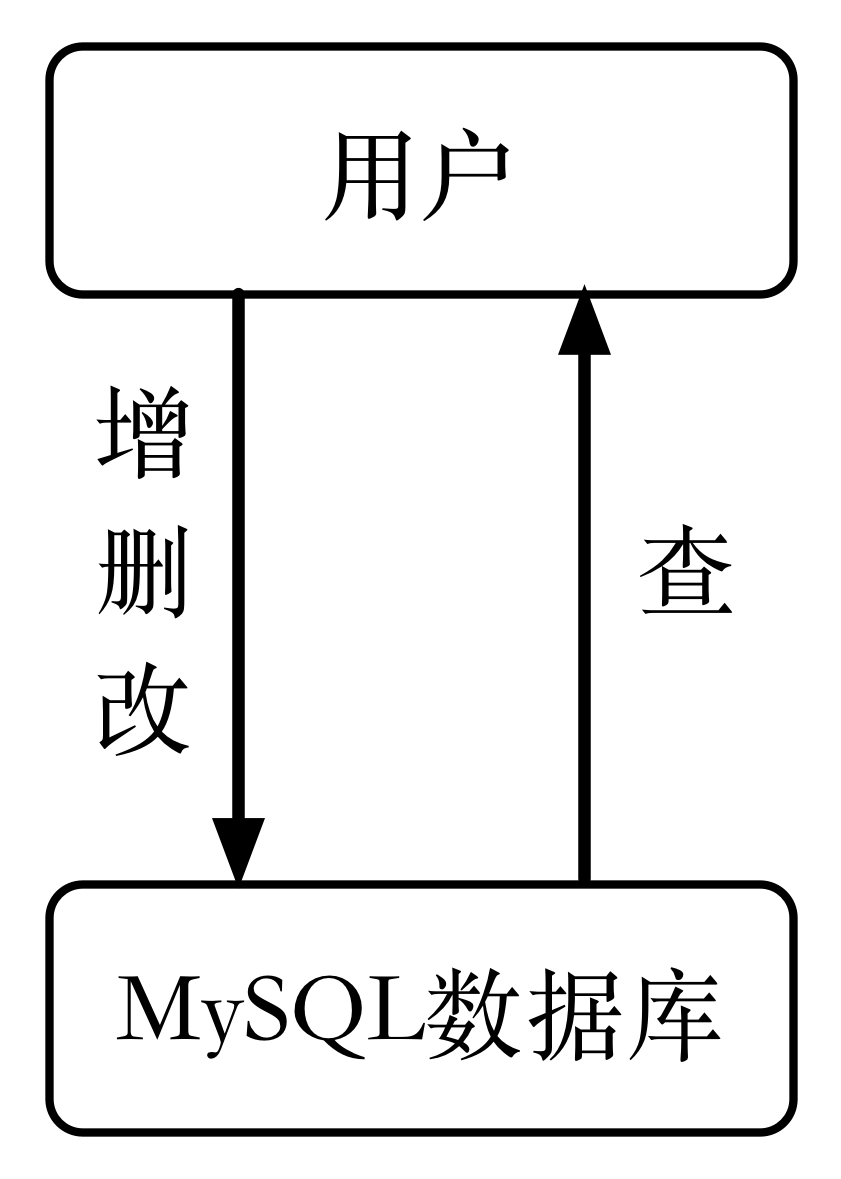
\includegraphics[width=1in]{chap03/couchbase1}
  \caption{通常数据操作流程}
  \label{fig:couchbase1}
\end{figure}
为了缓解数据库的压力,在数据的读取过程中将系统的基础数据读取到Couchbase缓存中,这样只需要对数据的基础数据进行一次读取即可完成数据的加载,降低了数据库的压力。通过缓存的数据操作流程参见图~\ref{fig:couchbase2}。
\begin{figure}[H] % use float package if you want it here
  \centering
  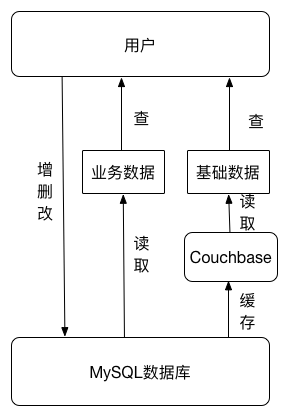
\includegraphics[width=1.7in]{chap03/couchbase2}
  \caption{通常数据操作流程}
  \label{fig:couchbase2}
\end{figure}
本论文中的WEB应用的数据包含基础数据和应用数据两部分,其中基础数据主要包括系统的基本配置数据、系统的常用变量数据、用户权限数据、枚举类型等相对固定的数据,这些数据在用户访问应用的时候只需要加载一次即可,不需要重复的从数据中读取,而应用数据则主要包含应用内的用户信息、商户信息、交易数据、库存数据等等不固定的数据,这些数据随着用户的时候会不断的发生变化,而且新的数据从数据库重新读取,这些数据在用户使用时需要多次加载。针对于以上不同数据的特点,将基础数据在用户首次登陆时加载到Couchbase缓存中,以后再读取时直接从缓存中读取。
\subsection{Couchbase安装}
\begin{enumerate}
\item 直接安装\cite{brown2012getting}

首先,通过浏览器访问\url{https://www.couchbase.com/nosql-databases/downloads}
,在页面中选择4.1.0版本、支持Red Hat 7平台的Couchbase Server安装文件couchbase-server-enterprise-4.1.0-centos7.x86\_64.rpm,将rpm文件复制到服务器中。或者直接在shell中通过
\begin{lstlisting}[language=bash,numbers=none]
$ wget https://packages.couchbase.com/releases/4.1.0/couchbase-server-enterprise-4.1.0-centos7.x86_64.rpm
\end{lstlisting}
命令将rpm安装文件下载到制定路径中。

然后,通过root用户访问Linux服务器,在终端中进入到couchbase安装文件所在路径,通过如下命令安装couchbase:
\begin{lstlisting}[language=bash,numbers=none]
$ rpm --install couchbase-server-enterprise-4.1.0-centos7.x86_64.rpm
\end{lstlisting}
安装完成后自动启动couchbase,并且会有如下提示信息:
\begin{lstlisting}[language=bash,numbers=none]
Warning: Transparent hugepages looks to be active and should not be.
Please look at http://bit.ly/1ZAcLjD as for how to PERMANENTLY alter this setting.
Minimum RAM required  : 4 GB
System RAM configured : 3.70 GB

Minimum number of processors required : 4 cores
Number of processors on the system    : 1 cores

Reloading systemd:                                         [  OK  ]
Starting couchbase-server (via systemctl):                 [  OK  ]

You have successfully installed Couchbase Server.
Please browse to http://iZ257vyhrvzZ:8091/ to configure your server.
Please refer to http://couchbase.com for additional resources.

Please note that you have to update your firewall configuration to
allow connections to the following ports: 11211, 11210, 11209, 4369,
8091, 8092, 8093, 9100 to 9105, 9998, 18091, 18092, 11214, 11215 and
from 21100 to 21299.

By using this software you agree to the End User License Agreement.
See /opt/couchbase/LICENSE.txt.
\end{lstlisting}
couchbase默认安装位置为“/opt/couchbase/”

\item Docker安装\cite{merkel2014docker}

\begin{lstlisting}[language=bash,numbers=none]
# 下载镜像
$ docker pull couchbase:4.1.0
# 运行容器
$ docker run -d --name db -p 8091-8094:8091-8094 -p 11210:11210 couchbase
\end{lstlisting}

\end{enumerate}
Couchbase安装完成后,需要在阿里云的安全策略中配置外网访问的端口和应用访问的端口,相关配置参见\ref{cha:Monitor-aliyun}
\subsection{Couchbase集群配置}
Couchbase服务器及可以单独运行,也可以将多个服务器组成一个集群,作为集群来运行。通过Couchbase集群,可以实现缓存数据的分布式存储及负载均衡,提升缓存的高可用以及系统的性能。

Couchbase数据分布是按计算分配到多个节点上,每个节点都储存两部分数据有效数据和副本数据,客户端对数据的操作主要是按照节点中对应的有效数据进行操作,执行压力会部分到不同的节点,如~\ref{fig:couchbase3}所示:
\begin{figure}[H] % use float package if you want it here
  \centering
  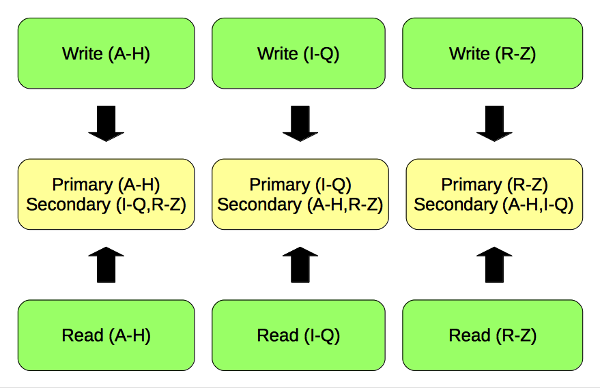
\includegraphics[width=3in]{chap03/couchbase3}
  \caption{Couchbase集群数据操作模型}
  \label{fig:couchbase3}
\end{figure}
Couchbase的集群管理是由erlang/otp进行集群通信管理,集群之间使用心跳机制进行监测服务器节点健康监测,配置参数信息是同步到每一个节点上进行储存。整个集群以vbucket为单位划分映射到不同服务器节点中进行储存,划分规则如下:
\begin{enumerate}
\item 均匀的分配有效vbucket和副本vbucket到不同服务器节点中;
\item 把有效数据与副本数据划分到不同物理节点中;
\item 在复制多份数据时,尽量有其它节点进行数据传播;
\item 扩展时,以最小化数据迁移量进行复制。
\end{enumerate}

在Couchbase负载均衡中,我们所操作的每一个bucket会逻辑划分为1024个vbucket,其数据的储存基于每个vbucket储存并且每个 vbucket都会映射到相对应的服务器节点,这种储存结构的方式叫做集群映射。如~\ref{fig:couchbase4}所示,当应用与Couchbase服务器交互时,会通过SDK的与 服务器数据进行交互,当应用操作某一个的bucket的key值时,在SDK中会通过哈希的方式计算,使用公式crc32(key)%1024确定key 值是属于1024个vbucket中的某个,然后根据vbucket所映射的节点服务器对数据进行操作。
\begin{figure}[H] % use float package if you want it here
  \centering
  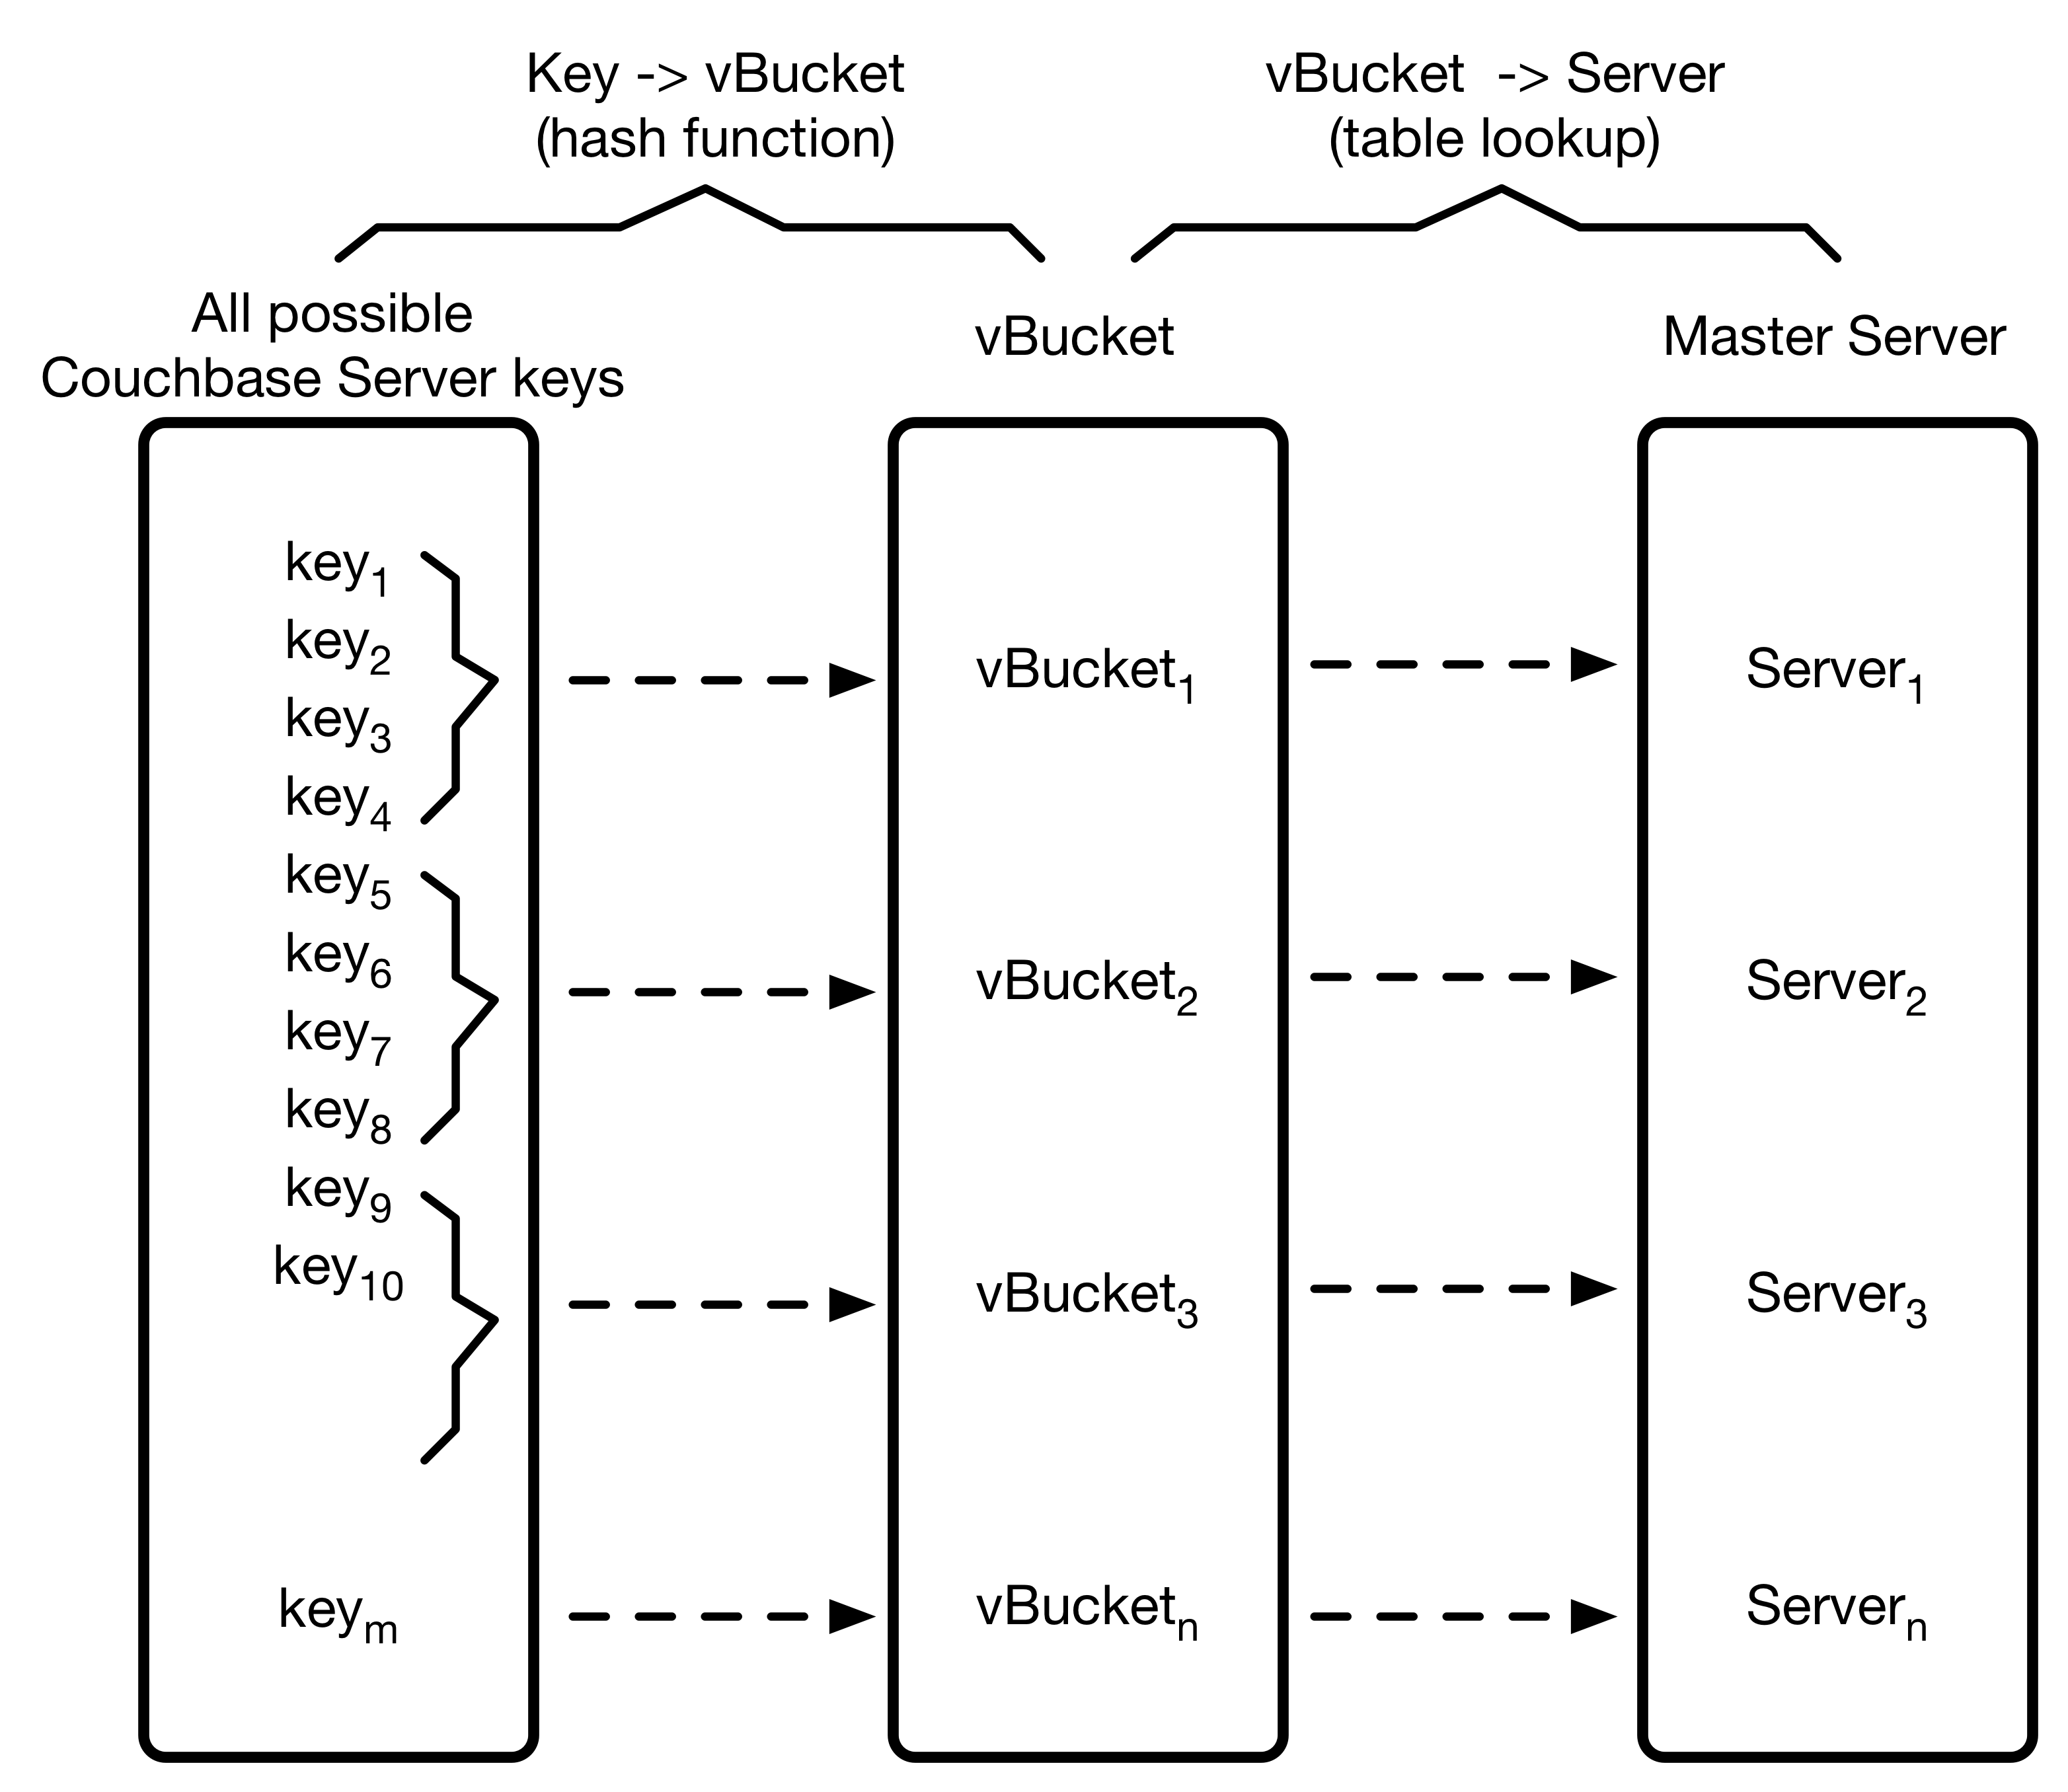
\includegraphics[width=3in]{chap03/couchbase4}
  \caption{Couchbase负载均衡模型}
  \label{fig:couchbase4}
\end{figure}
在设置标签页中的集群标签页下新建和配置集群信息
\begin{figure}[H] % use float package if you want it here
  \centering
  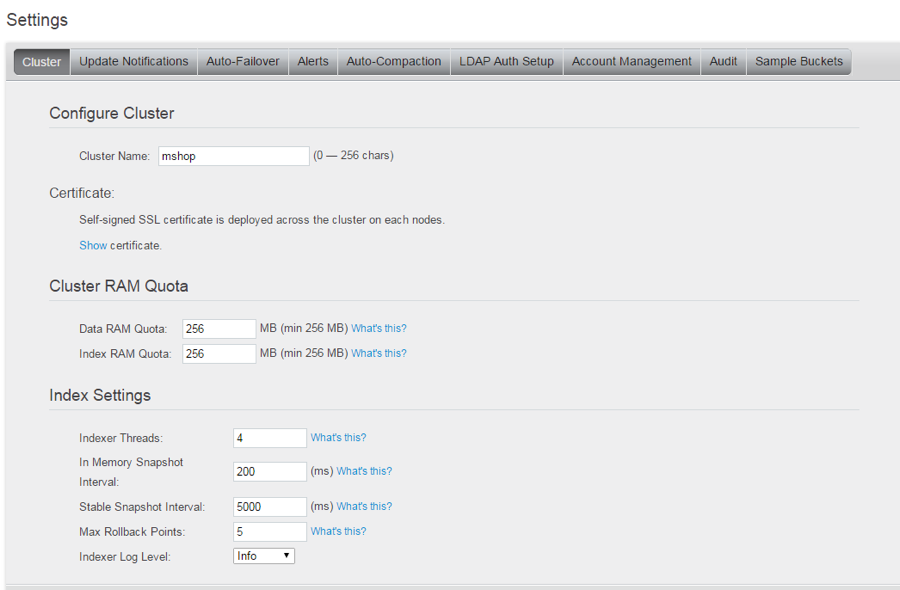
\includegraphics[width=3in]{chap03/couchbase5}
  \caption{Couchbase创建集群}
  \label{fig:couchbase5}
\end{figure}
在服务器节点标签页下新增服务器节点
\begin{figure}[H] % use float package if you want it here
  \centering
  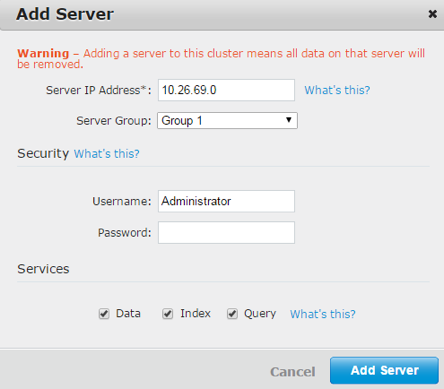
\includegraphics[width=3in]{chap03/couchbase6}
  \caption{Couchbase增加节点}
  \label{fig:couchbase6}
\end{figure}
增加完服务器节点后可以看到集群的基本信息
\begin{figure}[H] % use float package if you want it here
  \centering
  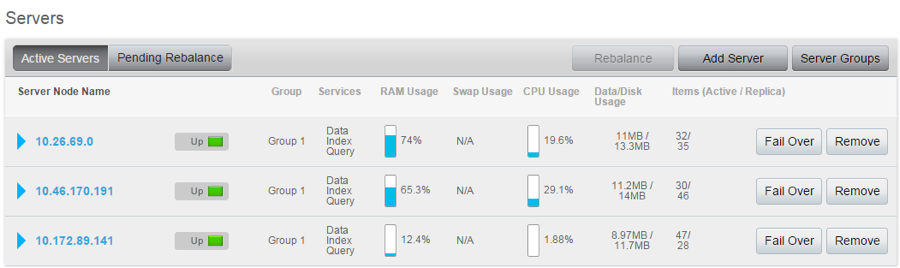
\includegraphics[width=3in]{chap03/couchbase7}
  \caption{Couchbase集群概览}
  \label{fig:couchbase7}
\end{figure}

% \subsection{Couchbase数据存取配置}
% \begin{enumerate}
% \item 启用couchbase
% 在项目的配置文件中增加config-couchbase的配置文件,并增加配置文件如下:
% \begin{lstlisting}[language=Java4]
% couchBase.maxWait=6000
% couchBase.maxclientPoolSize=2
% couchBase.minClientPoolSize=2
% couchBase.clientIncrease=1
% couchBase.bucketName=default
% couchBase.server=localhost:8091
% couchBase.serverPwd=
% # if use couchbase
% couchBase.inUsed=1
% \end{lstlisting}
% 在spring.xml文件中增加Couchbase的链接项和配置项。
% \item 数据存储

% \item 数据更新
% \end{enumerate}
\subsection{Couchbase缓存对系统性能影响}
通过ab命令对使用应用进行压力测试,在开启couchbase和关闭couchbase的情况下分别模拟5万个请求,每次并发10个请求来对比缓存对系统性能的影响:
\begin{lstlisting} [language=bash]
$ ab -n 50000 -c 10 -k http://test.hics.hisense.com:8081/client/mnsindex.html
This is ApacheBench, Version 2.3 <$Revision: 1748469 $>
Copyright 1996 Adam Twiss, Zeus Technology Ltd, http://www.zeustech.net/
Licensed to The Apache Software Foundation, http://www.apache.org/

Benchmarking test.hics.hisense.com (be patient)
Completed 5000 requests
Completed 10000 requests
Completed 15000 requests
Completed 20000 requests
Completed 25000 requests
Completed 30000 requests
Completed 35000 requests
Completed 40000 requests
Completed 45000 requests
Completed 50000 requests
Finished 50000 requests


Server Software:        nginx/1.9.12
Server Hostname:        test.hics.hisense.com
Server Port:            8081

Document Path:          /client/mnsindex.html
Document Length:        36028 bytes

Concurrency Level:      10
Time taken for tests:   206.318 seconds
Complete requests:      50000
Failed requests:        0
Keep-Alive requests:    49504
Total transferred:      1816897520 bytes
HTML transferred:       1801400000 bytes
Requests per second:    242.34 [#/sec] (mean)
Time per request:       41.264 [ms] (mean)
Time per request:       4.126 [ms] (mean, across all concurrent requests)
Transfer rate:          8599.92 [Kbytes/sec] received

Connection Times (ms)
              min  mean[+/-sd] median   max
Connect:        0    0   0.1      0       5
Processing:    20   41  19.1     38    1146
Waiting:       16   31   8.9     30    1058
Total:         20   41  19.2     38    1147

Percentage of the requests served within a certain time (ms)
  50%     38
  66%     44
  75%     47
  80%     49
  90%     54
  95%     62
  98%     75
  99%     86
 100%   1147 (longest request)
\end{lstlisting}
\begin{lstlisting} [language=bash]
$ ab -n 50000 -c 10 -k http://test.hics.hisense.com/client/mnsindex.html
This is ApacheBench, Version 2.3 <$Revision: 1748469 $>
Copyright 1996 Adam Twiss, Zeus Technology Ltd, http://www.zeustech.net/
Licensed to The Apache Software Foundation, http://www.apache.org/

Benchmarking test.hics.hisense.com (be patient)
Completed 5000 requests
Completed 10000 requests
Completed 15000 requests
Completed 20000 requests
Completed 25000 requests
Completed 30000 requests
Completed 35000 requests
Completed 40000 requests
Completed 45000 requests
Completed 50000 requests
Finished 50000 requests


Server Software:        Apache-Coyote/1.1
Server Hostname:        test.hics.hisense.com
Server Port:            80

Document Path:          /client/mnsindex.html
Document Length:        36028 bytes

Concurrency Level:      10
Time taken for tests:   247.137 seconds
Complete requests:      50000
Failed requests:        0
Keep-Alive requests:    49505
Total transferred:      1814097525 bytes
HTML transferred:       1801400000 bytes
Requests per second:    202.32 [#/sec] (mean)
Time per request:       49.427 [ms] (mean)
Time per request:       4.943 [ms] (mean, across all concurrent requests)
Transfer rate:          7168.40 [Kbytes/sec] received

Connection Times (ms)
              min  mean[+/-sd] median   max
Connect:        0    0   0.1      0      12
Processing:    21   49  17.5     45     528
Waiting:       17   27  12.0     24     504
Total:         21   49  17.6     45     528

Percentage of the requests served within a certain time (ms)
  50%     45
  66%     49
  75%     51
  80%     53
  90%     63
  95%     69
  98%     88
  99%    104
 100%    528 (longest request)
\end{lstlisting}
\section{Tomcat高并发APR优化}
Tomcat对用户请求的处理方式有BIO、NIO以及APR三种方式,其中BIO模式为Tomcat的默认处理方式\cite{vukotic2011securing}。

BIO模式是一种阻塞式I/O操作,这种模式表示Tomcat使用的是传统Java I/O操作。在这种模式下对于每个请求都要创建一个线程来处理,线程开销较大,不能处理高并发的场景,在三种模式中性能也最低。启动tomcat看到如图~\ref{fig:tomcat1}所示日志,表示使用的是BIO模式:
\begin{figure}[H] % use float package if you want it here
  \centering
  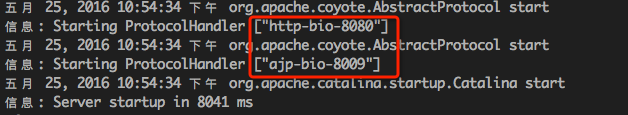
\includegraphics[width=3in]{chap03/tomcat1}
  \caption{BIO模式日志}
  \label{fig:tomcat1}
\end{figure}
NIO模式是Java SE 1.4及后续版本提供的一种新的I/O操作方式。该模式是一个基于缓冲区、并能提供非阻塞I/O操作的Java API,它拥有比传统I/O操作(bio)更好的并发运行性能。启动tomcat看到如图~\ref{fig:tomcat2}所示日志,表示使用的是NIO模式:
\begin{figure}[H] % use float package if you want it here
  \centering
  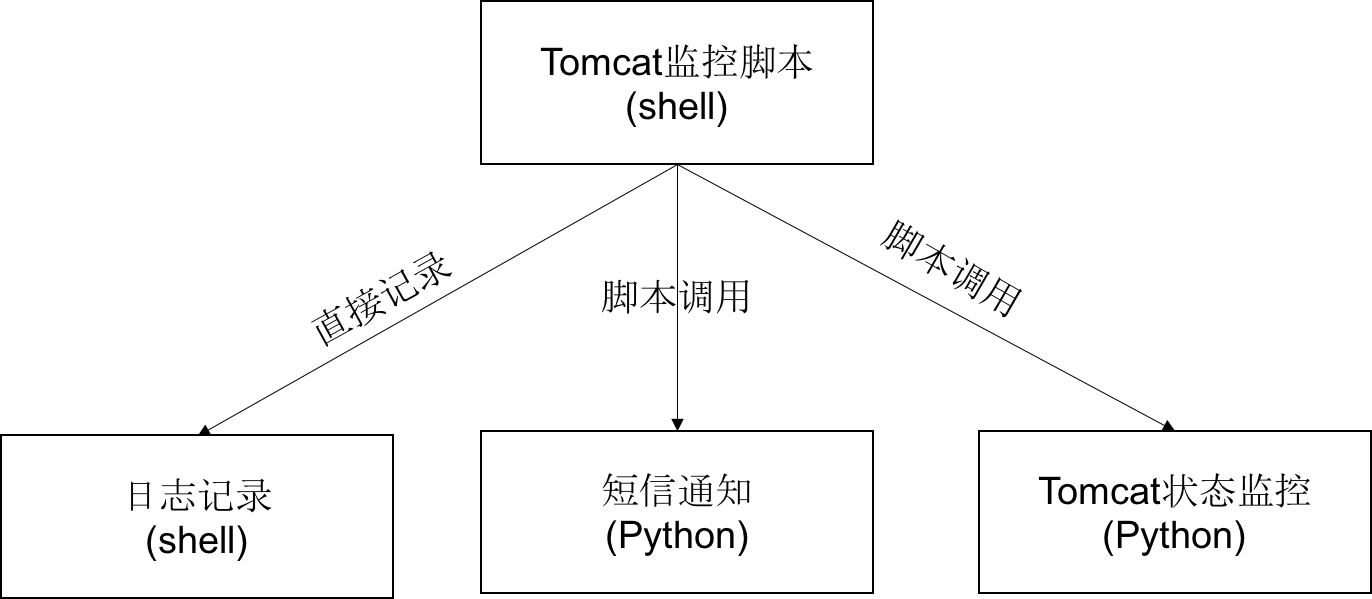
\includegraphics[width=3in]{chap03/tomcat2}
  \caption{NIO模式日志}
  \label{fig:tomcat2}
\end{figure}
APR模式是从操作系统级别解决异步IO问题,大幅度的提高服务器的处理和响应性能, 也是Tomcat运行高并发应用的首选模式。启动tomcat看到如图~\ref{fig:tomcat3}所示日志,表示使用的是NIO模式:
\begin{figure}[H] % use float package if you want it here
  \centering
  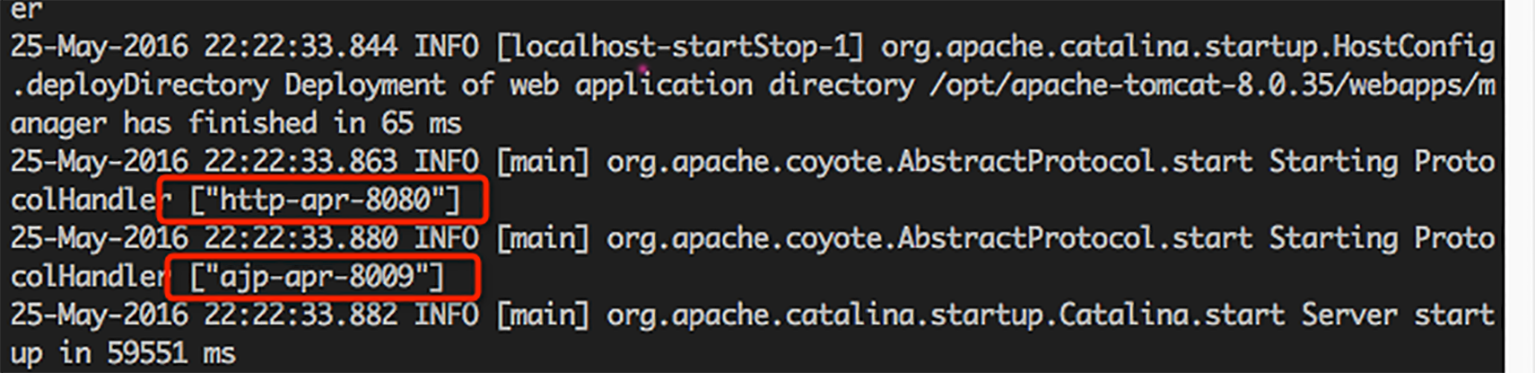
\includegraphics[width=3in]{chap03/tomcat3}
  \caption{APR模式日志}
  \label{fig:tomcat3}
\end{figure}
考虑到应用在大量用户访问的情况下必然会出现高并发的现象,因此调整Tomcat的请求处理方式为APR模式对于提升系统的高并发处理能力时非常必要的\cite{蒋文旭2012大型高并发}。

APR(Apache Portable Runtime)是一个高可移植库,它是Apache HTTP Server 2.x的核心。APR有很多用途,包括访问高级IO功能(例如sendfile,epoll和OpenSSL),OS级别功能(随机数生成,系统状态等等),本地进程管理(共享内存,NT管道和UNIX sockets)。这些功能可以使Tomcat作为一个通常的前台WEB服务器,能更好地和其它本地web技术集成,总体上让Java更有效率作为一个高性能web服务器平台而不是简单作为后台容器。

在产品环境中,特别是直接使用Tomcat做WEB服务器的时候,应该使用Tomcat Native来提高其性能,要测APR给tomcat带来的好处最好的方法是在慢速网络上(模拟Internet),将Tomcat线程数开到300以上的水平,然后模拟一大堆并发请求。

如果不配APR,基本上300个线程狠快就会用满,以后的请求就只好等待。但是配上APR之后,并发的线程数量明显下降,从原来的300可能会马上下降到只有几十,新的请求会毫无阻塞的进来。
在局域网环境测,就算是400个并发,也是一瞬间就处理/传输完毕,但是在真实的Internet环境下,页面处理时间只占0.1\%都不到,绝大部分时间都用来页面传输。如果不用APR,一个线程同一时间只能处理一个用户,势必会造成阻塞。所以生产环境下用apr是非常必要的。
\subsection{开启APR模式}

\subsection{APR模式对于系统性能的影响}
\section{Docker分布式优化}
随着用户数量的增加以及应用业务的扩展,目前WEB应用的数据库服务器已经由一台服务器扩展为两台服务器,应用服务器也已经由一台服务器扩展为两台服务器,加上目前的测试服务器,一共有5台服务器服务于一个WEB应用,而且在未来的发展过程中,无论是数据节点还是应用节点,数量肯定时不断增加的。在节点不断增加的情况下,如何快速部署一个数据库节点或者一个应用节点必然是运维人员在新增节点时必须要面对的问题。

在新增节点上部署服务的方式主要有直接安装以及容器技术两种方式,其中直接安装的方式依靠手动的在服务器中安装各种库以及依赖,然后安装应用软件病进行配置,这种方式在快速部署一个节点的过程中的劣势非常明显。

目前实现快速部署新增节点的解决方案主要有虚拟机技术和容器技术两种技术,其中传统虚拟机技术是虚拟出一套硬件后,在其上运行一个完整操作系统,在该系统上再运行所需应用进程,如图~\ref{fig:docker1}所示;而容器内的应用进程直接运行于宿主的内核,容器内没有自己的内核,而且也没有进行硬件虚拟。因此容器要比传统虚拟机更为轻便如图~\ref{fig:docker2}所示\cite{刘熙2016基于}。

\begin{figure}[H] % use float package if you want it here
  \centering
  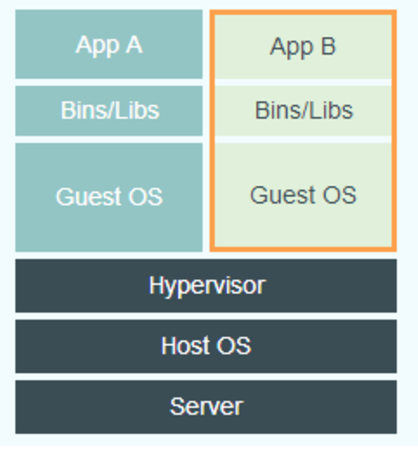
\includegraphics[width=3in]{chap03/docker1}
  \caption{传统虚拟机模型}
  \label{fig:docker1}
\end{figure}
\begin{figure}[H] % use float package if you want it here
  \centering
  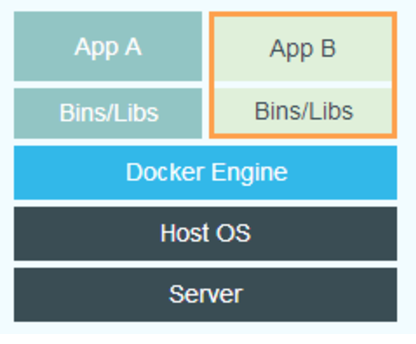
\includegraphics[width=3in]{chap03/docker2}
  \caption{Docker容器模型}
  \label{fig:docker2}
\end{figure}
同传统的虚拟机技术相比,Docker容积技术具有非常多的优势,这也是本论文中使用Docker技术作为WEB应用开发过程中服务器扩展的主要技术。
\begin{itemize}
\item 更高效的利用系统资源

由于容器不需要进行硬件虚拟以及运行完整操作系统等额外开销,Docker 对系统资源的利用率更高。无论是应用执行速度、内存损耗或者文件存储速度,都要比传统虚拟机技术更高效。因此,相比虚拟机技术,一个相同配置的主机,往往可以运行更多数量的应用。
\item 更快速的启动时间

传统的虚拟机技术启动应用服务往往需要数分钟,而 Docker 容器应用,由于直接运行于宿主内核,无需启动完整的操作系统,因此可以做到秒级、甚至毫秒级的启动时间。大大的节约了开发、测试、部署的时间。
\item 一致的运行环境

开发过程中一个常见的问题是环境一致性问题。由于开发环境、测试环境、生产环境不一致,导致有些 bug 并未在开发过程中被发现。而 Docker 的镜像提供了除内核外完整的运行时环境,确保了应用运行环境一致性,从而不会再出现 “这段代码在我机器上没问题啊” 这类问题。
\item 持续交付和部署

对开发和运维(DevOps)人员来说,最希望的就是一次创建或配置,可以在任意地方正常运行。

使用 Docker 可以通过定制应用镜像来实现持续集成、持续交付、部署。开发人员可以通过 Dockerfile 来进行镜像构建,并结合 持续集成(Continuous Integration) 系统进行集成测试,而运维人员则可以直接在生产环境中快速部署该镜像,甚至结合 持续部署(Continuous Delivery/Deployment) 系统进行自动部署。

而且使用 Dockerfile 使镜像构建透明化,不仅仅开发团队可以理解应用运行环境,也方便运维团队理解应用运行所需条件,帮助更好的生产环境中部署该镜像。
\item 更轻松的迁移

由于 Docker 确保了执行环境的一致性,使得应用的迁移更加容易。Docker 可以在很多平台上运行,无论是物理机、虚拟机、公有云、私有云,甚至是笔记本,其运行结果是一致的。因此用户可以很轻易的将在一个平台上运行的应用,迁移到另一个平台上,而不用担心运行环境的变化导致应用无法正常运行的情况。
\item 更轻松的维护和扩展

Docker 使用的分层存储以及镜像的技术,使得应用重复部分的复用更为容易,也使得应用的维护更新更加简单,基于基础镜像进一步扩展镜像也变得非常简单。此外,Docker 团队同各个开源项目团队一起维护了一大批高质量的官方镜像,既可以直接在生产环境使用,又可以作为基础进一步定制,大大的降低了应用服务的镜像制作成本。
\item 对比传统虚拟机总结
\begin{table}[H]
  \centering
  \begin{minipage}[t]{0.8\linewidth} % 如果想在表格中使用脚注,minipage是个不错的办法
  % \caption[模板文件]{模板文件。如果表格的标题很长,那么在表格索引中就会很不美
  %   观,所以要像 chapter 那样在前面用中括号写一个简短的标题。这个标题会出现在索
  %   引中。}
  \label{tab:docker-compare}
    \begin{tabularx}{\linewidth}{lXX|}
      \toprule[1.5pt]
      {\heiti 对比参数} & {\heiti 容器技术} & {\heiti 虚拟机技术}\\\midrule[1pt]
      启动时间  &  秒级 & 分钟级 \\
      硬盘使用  &  一般为MB  &  一般为GB\\
      应用性能  &  接近原生  &  弱于\\
      系统支持量 & 单机支持上千个容器 & 一般几十个\\
      \bottomrule[1.5pt]
    \end{tabularx}
  \end{minipage}
\end{table}
\end{itemize}

\subsection{使用Docker Compose管理Docker容器}
在Docker安装完成后,可以通过docker pull 命令下载相应的镜像,通过ducker run运行镜像,生成一个运行中的容器。除了通过ducker run命令运行容器以外,还可以通过Docker Compose工具来快速在集群中部署分布式应用以及容器的管理工作。

使用Docker Compose 项目是 Docker 官方的开源项目,负责实现对 Docker 容器集群的快速编排。它的定位是 “定义和运行多个 Docker 容器的应用(Defining and running multi-container Docker applications),它允许用户通过一个单独的 docker-compose.yml 模板文件(YAML 格式)来定义一组相关联的应用容器为一个项目(project)。

Compose 中有两个重要的概念:
\begin{itemize}
\item 服务(service):一个应用的容器,实际上可以包括若干运行相同镜像的容器实例。
\item 项目(project):由一组关联的应用容器组成的一个完整业务单元,在 docker-compose.yml 文件中定义。
\end{itemize}
Compose 的默认管理对象是项目,通过子命令对项目中的一组容器进行便捷地生命周期管理。

Compose 项目由 Python 编写,实现上调用了 Docker 服务提供的 API 来对容器进行管理。因此,只要所操作的平台支持 Docker API,就可以在其上利用 Compose 来进行编排管理。

对于Mysql可以通过修改docker-compose.yml文件来实现数据库镜像的运行以及容器的相关控制:
\begin{lstlisting} [language=sh,numbers=none]
version: '2'
services:
    mysql_master:
        image: docker.io/mysql
        restart: always
        container_name: mysql-master
        ports:
            - "3306:3306"
        volumes:
            - ./master/conf:/etc/mysql/conf.d
            - ./master/data:/var/lib/mysql
            - /etc/localtime:/etc/localtime:ro
        environment:
            MYSQL_ROOT_PASSWORD: "*********"
    mysql_slave:
        image: docker.io/mysql
        restart: always
        container_name: mysql-slave
        ports:
            - "3307:3306"
        volumes:
            - ./slave/conf:/etc/mysql/conf.d
            - ./slvae/data:/var/lib/mysql
            - /etc/localtime:/etc/localtime:ro
        environment:
            MYSQL_ROOT_PASSWORD: "*********"
\end{lstlisting}
上述配置文件通过运行docker.io/mysql镜像生成两个mysql容器,其中一个的端口为3306,另一个的端口为3307,这样能够很方面的创建两个容器。同样,根据这个方法也可以创建多个相互关联的容器,比如Tomcat和Mysql的相互关联。
\subsection{应用容器化现状}
根据现阶段的项目开发和服务器运维需求,已经在生产环境的两个数据库服务器中通过Docker实现了Mysql数据库容器的运行,在生产环境的两个应用服务器中实现了Couchbase应用的容器化,在测试环境的服务器中实现了测试环境数据库、测试环境Couchbase、生产环境服务器Couchbase节点、生产环境延时备份数据库的容器化。这样,当部署一个新的服务器节点的时候,可以通过Docker容器快速部署数据库应用、Couchbase应用。

目前考虑到Tomcat在运行过程中需要面临频繁修改的配置文件、库文件以及其他工具的配置等问题,Docker Hub中官方的Tomcat镜像无法满足项目开发的实际需求,暂时没有实现Tomat的容器化。为了后期Tomcat的容器化,目前也正在预研通过Dockerfile定制镜像的方式定制符合项目需求的Tomcat镜像,预研工作完成后即进行Tomcat的容器话需求。

由于Docker Hub的官方镜像服务器在国外,在本地服务器中通过docker pull 命令下载镜像的速度太慢,难以满足快速部署的需求,故在生产环境的一个服务器节点中部署了本地的Docker 镜像源,后期在新节点可以通过docker pull本地的镜像源来下载官方的以及定制的docker镜像。
\section{SLB负载均衡优化}

随着用户访问的增加以及服务高可用的需求,单个应用节点无法满足项目的需求,因此需要通过增加应用服务器节点来实现WEB应用的高可用,并且通过负载均衡将用户的请求转发到不同的服务器,降低单个服务器节点的压力。

负载均衡(Load balancing)是一种计算机网络技术,用来在多个计算机(计算机集群)、网络连接、CPU、磁盘驱动器或其他资源中分配负载,以达到最佳化资源使用、最大化吞吐率、最小化响应时间、同时避免过载的目的。

使用带有负载均衡的多个服务器组件,取代单一的组件,可以通过冗余提高可靠性。

负载平衡最重要的一个应用是利用多台服务器提供单一服务,这种方案有时也称之为服务器农场。通常,负载平衡主要应用于Web网站,大型的Internet Relay Chat网络,高流量的文件下载网站,NNTP(Network News Transfer Protocol)服务和DNS服务。现在负载平衡器也开始支持数据库服务,称之为数据库负载平衡器。
对于互联网服务,负载平衡器通常是一个软体程序,这个程序侦听一个外部端口,互联网用户可以通过这个端口来访问服务,而作为负载平衡器的软体会将用户的请求转发给后台内网服务器,内网服务器将请求的响应返回给负载平衡器,负载平衡器再将响应发送到用户,这样就向互联网用户隐藏了内网结构,阻止了用户直接访问后台(内网)服务器,使得服务器更加安全,可以阻止对核心网络栈和运行在其它端口服务的攻击。
当所有后台服务器出现故障时,有些负载平衡器会提供一些特殊的功能来处理这种情况。例如转发请求到一个备用的负载平衡器、显示一条关于服务中断的消息等。负载平衡器使得IT团队可以显著提高容错能力。它可以自动提供大量的容量以处理任何应用程序流量的增加或减少\cite{wei2010system}。

负载均衡的主要特点有:
\begin{enumerate}
\item 解决并发压力,提高应用处理性能(增加吞吐量,加强网络处理能力);
\item 提供故障转移,实现高可用;
\item 通过添加或减少服务器数量,提供网站伸缩性(扩展性);
\item 安全防护;(负载均衡设备上做一些过滤,黑白名单等处理);
\end{enumerate}

考虑到本项目中的所有服务器节点均为阿里云云服务器,故选择通过使用阿里云的负载均衡服务器服务(SLB)来进行应用的负载均衡,通过创建一个负载均衡服务,即可获取到一个公网的IP,通过配置监听,将WEB应用的http协议端口(80)和https(443)协议分别转发到生产环境各应用服务器节点的Tomcat对应端口,通过配置服务器节点的权重来决定负载均衡在转发用户请求时向后端服务器转发的比重。

\section{本章总结}
本章主要是对WEB应用的应用性能进行优化,主要包括通过配置Couchbase缓存机制,将应用的基础数据加载到缓存中,在提升应用的相应速度的同时降低了数据库的压力;通过调整Tomcat的请求处理方式为APR模式,提升Tomcat对于高并发的处理能力;通过Docker容器编排技术将应用通过容器的方式运行在服务器中,实现了节点快速部署应用的能力;通过配置应用负载均衡,在提升服务的高可用性的同时降低了服务器节点的压力。
